\documentclass{article}
\usepackage{malmacros}
\begin{document}

\section{Hyperparameters and Gridsearch}
In this section, grid search will be explored. It will be discussed how it works, and a grid search using an SGD classifier is implemented where different hy-perparamaters are searched through to get the best parameters for the classifier. After, the random search will be used instead. Lastly, a search quest is performed on the mnist data set.

\subsection{Qa Explain GridSearchCV}
A model can have several hyperparameters: these are parameters that are set by the invoker of the model, and are not found by the model itself. A \textit{grid search} will help find the best model for a given data set.
\\ \\
The code consists of two sections. The first part consist of several functions: SearchReport(), ClassificationReport(), FullReport() and LoadAndSetupData(). It will print the best parameters found, the best score and the best index. The best constructor is also printed. Then it will iterate through every result in the model and show the respective score for every iteration the grid search has done. SearchReport() has a function, GetBestModelCTOR(), that will receive a model and the best parameters found. It will then return the best parameters in a pretty format as a string. SearchReport() will lastly return the results  as a string.
\\ \\
ClassificationReport() will print a classification report by  calling predict() on the model with some test data, and show a classification report based on this. It will return a precision, recall, f1-score and support.
\\ \\
FullReport() will simply call SearchReport() and ClassificationReport() and also show the time used to find the best hyper parameters.
\\ \\
Lastly, LoadAndSetupData() will simply get either moon, mnist or iris data, split it into test and train data, and return this.
\\ \\
The more important bit of the code is the next section that will actually perform the grid search. This is seen below.

\begin{pyminted}
# Setup data
X_train, X_test, y_train, y_test = LoadAndSetupData('iris') # or 'moon', or 'mnist'

# Setup search parameters
model = svm.SVC(gamma="scale")

tuning_parameters = {
    'kernel':('linear', 'rbf'), 
    'C':[1, 10]
}

CV=5
VERBOSE=0

# Run GridSearchCV for the model
start = time()
grid_tuned = GridSearchCV(model, tuning_parameters, cv=CV, scoring='f1_micro', verbose=VERBOSE, n_jobs=-1, iid=True)
grid_tuned.fit(X_train, y_train)
t = time()-start

# Report result
b0, m0= FullReport(grid_tuned , X_test, y_test, t)
\end{pyminted}

The iris data is loaded into a train and test set, and SVC (\textit{Support Vector Classification}), is used as the model. Tuning parameters will be defined. This is fed into the GridSearchCV to let it know what it has to set the various parameters to in each search. So it will try every combination of the 2 parameters with the various combinations of kernel = linear or rbf and C = 1 or 10. This at first gives 4 different combinations to fit on X-train and y-train, when tuning the model. But an added CV=5, sets the model to run cross validation with 5-kfolds, which means that each model with the 4 combinations will be trained 5 times, leading to a total of 40 rounds of training. To measure how long it takes for the GridSearchCV to iterate through every combination, a timer is started with time() and ended after the search is done.  The GridSearchCV will find the highest f1 micro score. 
\\ \\
A f1 micro score can be used to calculate the f1 score of a multi-class, which the iris data set is (0, 1 or 2). This means it will count the metrics globally by counting the true positive, false negatives and false positive, and then it takes the average of these and returns it as a score. This gives each sample-class pair an equal contribution to the overall metric. The \textit{n\_jobs} parameter tells how many processing jobs it should be scheduled and run in parallel. With the value set to -1 means using the total number of processors available on the system.
\\ \\
A full report of the iterations, best parameters, the score, a classification report etc is printed. Figure \ref{fig:les6-grid-a}
contains the detailed classification report, the CTOR for best model and a summary of the best score and parameters.

\begin{figure}[H]
  \centering
    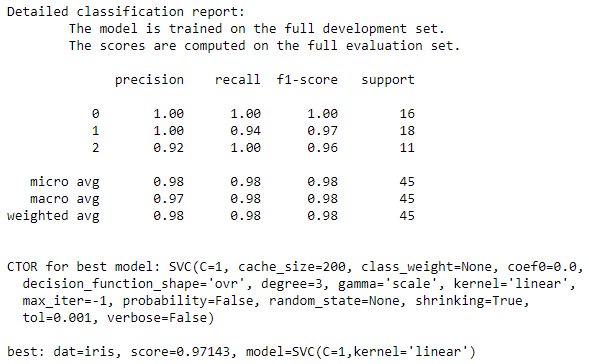
\includegraphics[width=0.8\textwidth]{les6-grid-a}
    \caption{Detailed classification report and summary of the best parameters of the simple grid search}
    \label{fig:les6-grid-a}
\end{figure}

It classifies C =  1 and kernel = linear as the best parameters. It has a rather good f1 micro score of 0.97. The precision, recall and f1-score of the individual classes is also very good, only misses a few instances in the data set. 

\subsection{Qb Hyperparameter Grid Search using an SDG classifier}
In this section, the same code is implemented, but now with an SGDClassifier, and many more hyperparameters and values for the grid search to search through.

\begin{pyminted}

# Setup data
X_train, X_test, y_train, y_test = LoadAndSetupData('iris') # or 'moon', or 'mnist'

# Setup search parameters
model = SGDClassifier(random_state=42)

tuning_parameters = {
    'penalty':['l2', 'l1', 'elasticnet'],
    'alpha':[0, 0.0001, 0.001, 0.01, 1],
    'learning_rate':['constant', 'adaptive'],
    'eta0':[0.001, 0.1, 0.5, 1, 10],
    'l1_ratio':[0, 0.01, 0.10, 0.5, 1],
    'max_iter':[10, 100, 1000, 10000],
    'tol':[0, 0.03, 0.0003, 0.00003]
}

CV=3
VERBOSE=0
# ...
# ...
# ...
\end{pyminted}

The code is very similiar to the previous, except the SGDClassifier is used (and has a random state = 42). Then a set of tuning hyper-parameters are defined, such as penalty, alpha, learning rate ... These will all be iterated through to find the best hyper-parameters. The result is shown in figure \ref{fig:les6-grid-a} and figure \ref{fig:les6-grid-b2}.

\begin{figure}[H]
  \centering
    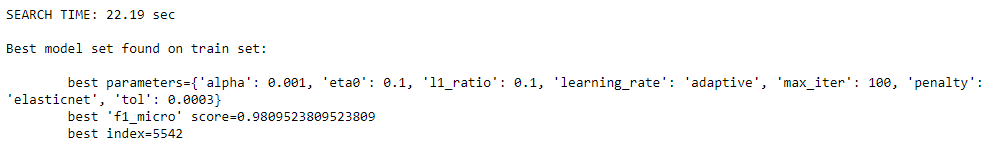
\includegraphics[width=1\textwidth]{les6-grid-b}
    \caption{Detailed classification report of the SGDClassifier search}
    \label{fig:les6-grid-b}
\end{figure}

\begin{figure}[H]
  \centering
    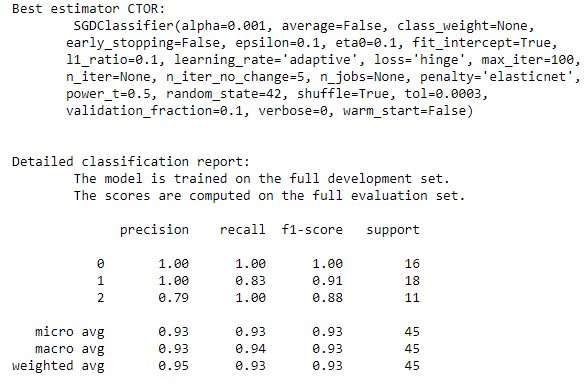
\includegraphics[width=0.9\textwidth]{les6-grid-b2}
    \caption{Detailed classification report of the SGDClassifier search}
    \label{fig:les6-grid-b2}
\end{figure}

\noindent
Since the grid search in Qa has to search through only 4 different combinations, with 5-folds, at total of 40 runs. The search only takes a few seconds to complete. The GridSearchCV will obviously take longer, the more parameters and various values of the individual parameters it has to search through. It will iterate through every option in the tuning parameters and find the best parameters that gives the highest f1 micro score. This is obvious to see, since this search trains 12000 different models and takes about 22.19 seconds to complete. The f1 micro score of the best classifier is calculated as 0,98 and the hyperparameters found are seen in figure \ref{fig:les6-grid-b2}. The precision, recall and f1-scores are also pretty good (the precision of 2 is a bit off though).

\subsection{Qc Hyperparameter Random Search using an SDG classifier}

Now we repeat the previous exercise but with this attempt using a randomized approach.
By using the Scikit-Learn's \textbf{RandomizedSearchCV}.
Most of the parameters are the same as before, but now with an added \textbf{n\_iter} = 20 which controls the amount model combinations that are tried and trained. A note to the addition of the \textbf{long\_version} parameter to \textbf{FullReport()} method. It is to shorten the output, as printing out the \textbf{f1\_micro} score for each of the 1200 trained models leads to quite the wall of text.

\begin{pyminted}
n_iter=20
start = time() # Starting the "timer".

# Setting the parameters for the randomized grid search.
random_tuned = RandomizedSearchCV(
    model, tuning_parameters, random_state=42, n_iter=20, cv=CV,
    scoring='f1_micro', verbose=VERBOSE, n_jobs=-1, iid=True)

# Fitting it on the training set.
random_tuned.fit(X_train, y_train)
t = time()-start # Getting a stop time for comparison.

# Report result
# !!! NOTE - Added the extra "long_version" parameter, to shorten the output.
b0, m0= FullReport(grid_tuned , X_test, y_test, t, long_version_false) # Keep the important parts
print('OK')
\end{pyminted}


\noindent
The results are primarily the same, but the very interesting thing to note: The search time is significantly lower! As can be seen in figure \ref{fig:les6-grid-c}. So with only 20 iterations/combinations run in only 0.13 seconds (using the GPU-cluster) we arived at the same result.

\begin{figure}[H]
  \centering
    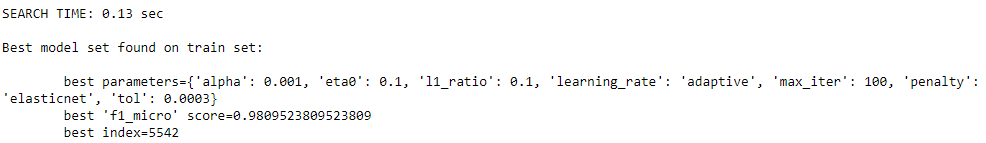
\includegraphics[width=0.7\textwidth]{les6-grid-c}
    \caption{Time report - for comparison with the previous normal GridSearch.}
    \label{fig:les6-grid-c}
\end{figure}

\subsubsection{Qd Search Quest}
In this section we want to perform a search quest. experimenting with finding the best models,
using different classifiers and parameters, trying to get the best result, though without using any of the TensorFlow or Keras models or any ANN's. Alo this time we are using the \textbf{MNIST} data set instead which is much bigger and heavyer than the previous iris set.

So first we load in the data and prepare the tuning parameters. And in the first example here,
a \textbf{DecisionTreeClassifier} is chosen.

\begin{pyminted}
# First loading in the data:
X_train, X_test, y_train, y_test = LoadAndSetupData('mnist') # or 'moon', or 'mnist'

# Trying a different classifier and setting up the tuning parameters.
from sklearn.tree import DecisionTreeClassifier
tree_model = DecisionTreeClassifier()

tuning_parameters = {
    'criterion': ('gini', 'entropy'),
    'splitter': ('best', 'random'),
    'min_samples_leaf': [1, 10, 30]
}

CV=3
VERBOSE=0

start = time()
grid_tuned = GridSearchCV(tree_model, tuning_parameters, cv=CV, scoring='f1_micro', verbose=VERBOSE, n_jobs=1, iid=True)
grid_tuned.fit(X_train, y_train)
t = time()-start

# Report result
b0, m0= FullReport(grid_tuned , X_test, y_test, t, long_version=False) # Keep the important parts
print('OK')
\end{pyminted}

\newpage
\noindent
The result is not great, the best average \textbf{f1\_micro} is only at a 86.27 percent. And the time it took to find the result was quite long.
155 seconds as it's shown in figure \ref{fig:les6-grid-d}.

\begin{figure}[H]
  \centering
    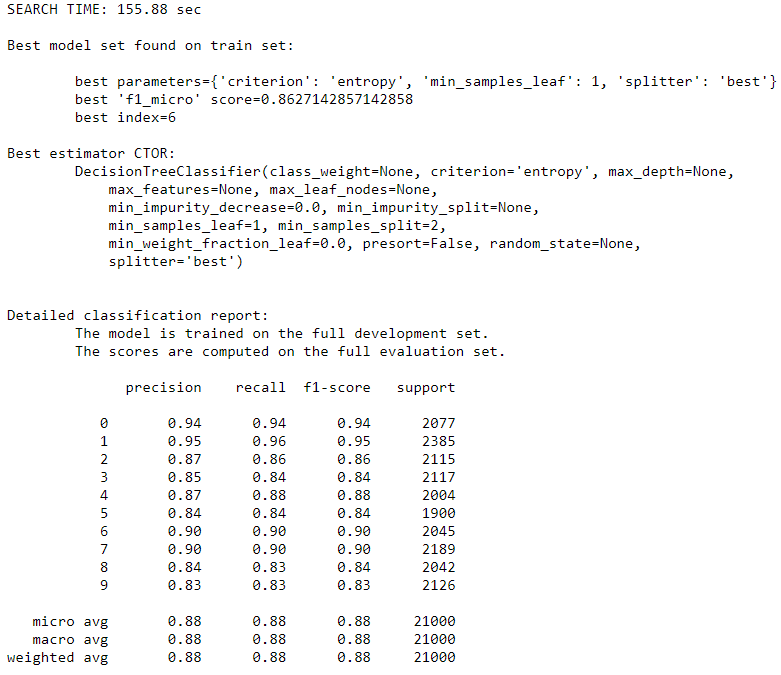
\includegraphics[width=0.8\textwidth]{les6-grid-d}
    \caption{Full report of the GridSearch for DecisionTreeClassifier.}
    \label{fig:les6-grid-d}
\end{figure}



\noindent
Testing with a randomized search gave the same result, even with the added parameters. 
But with a shorter search time of course.

\begin{pyminted}
# Now with a random search and slightly more parameters.
tuning_parameters = {
    'criterion': ('gini', 'entropy'),
    'splitter': ('best', 'random'),
    'min_samples_leaf': [1, 10, 30],
    'class_weight': ('balanced', None)
}

CV=3
VERBOSE=0

# start time and set the random search parameters
start = time()
random_tuned = RandomizedSearchCV(tree_model, tuning_parameters, random_state=42, n_iter=20, cv=CV,
    scoring='f1_micro', verbose=VERBOSE, n_jobs=-1, iid=True)

# fitting the random model.
random_tuned.fit(X_train, y_train)
t = time()-start

# Report result
b0, m0= FullReport(random_tuned , X_test, y_test, t, long_version=False) # Keep the important parts
print('OK')
\end{pyminted}

\noindent The full report output is shown in figure \ref{fig:les6-grid-d2}. Again note we have omitted the output of the \textbf{f1\_micro} score for each of the individually trained models. As it for the most part is uninteresting and just creates a huge wall of text on the output.
\begin{figure}[H]
  \centering
    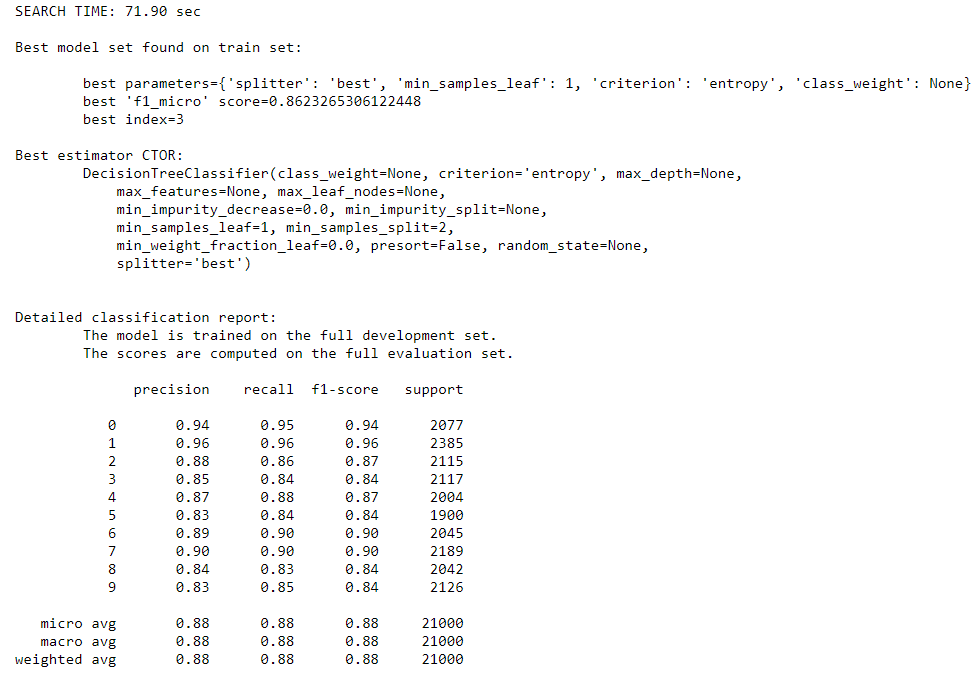
\includegraphics[width=1\textwidth]{les6-grid-d2}
    \caption{Full report of the RandomSearchCV for DecisionTreeClassifier.}
    \label{fig:les6-grid-d2}
\end{figure}


\noindent
Last we do another random search with the \textbf{SGDClassifier} with some other parameters that previous. This is to see if it does noticeably better than the DecisionTreeClassifier.

\begin{pyminted}
# Now we will try with the SGDClassifier we have used before and know well.
sgd_model = SGDClassifier(random_state=42)

#Defining the tuning parameters:
tuning_parameters = {
    'alpha': [0.0001, 0.001],
    'max_iter': [1,10,100],
    'learning_rate':('constant','optimal'),
    'eta0':[0.01, 0.02, 0.03]
}
CV=3
VERBOSE=0
# How ever only running it with random search as it takes forever running through mnist.
# even with a few parameters.

start = time()
sgd_random_tuned = RandomizedSearchCV(sgd_model, tuning_parameters, random_state=42, n_iter=20, cv=CV,
    scoring='f1_micro', verbose=VERBOSE, n_jobs=-1, iid=True)
# fitting the random model.
sgd_random_tuned.fit(X_train, y_train)
t = time()-start

# Report result
b0, m0= FullReport(sgd_random_tuned , X_test, y_test, t, long_version=False) # Keep the important parts
print('OK')
\end{pyminted}

\noindent
The results aren't impressive but it does slightly better score wise, but takes a lot longer than the DecisionTree did.
With a time of 258 seconds its not particularly fast, and only with an increased score of 0.6 percent.
But this is a good example when arguing whether precision is worth the resource cost.

\begin{figure}[H]
  \centering
    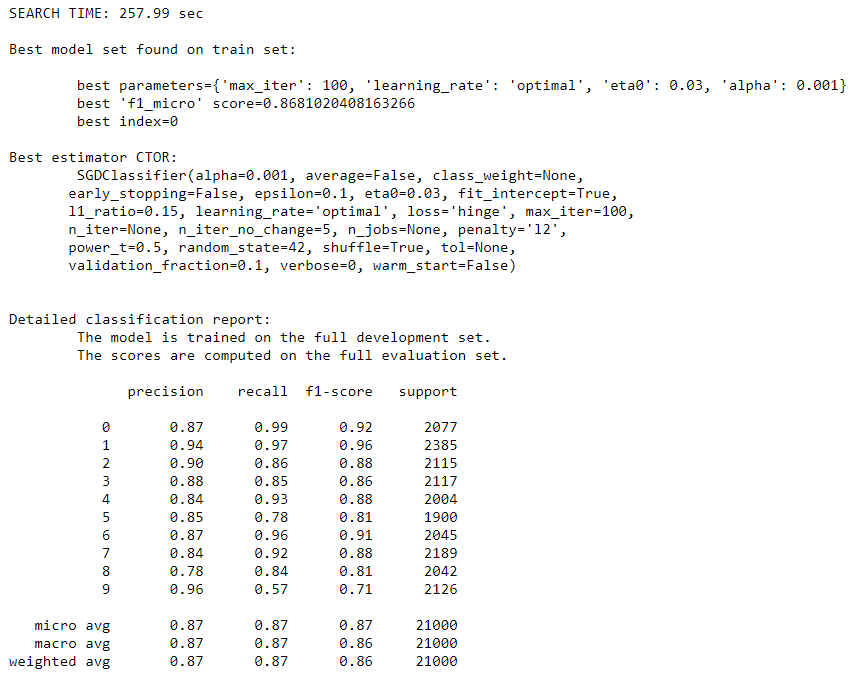
\includegraphics[width=1\textwidth]{les6-grid-d3}
    \caption{Full report of the RandomSearchCV for SGDClassifier.}
    \label{fig:les6-grid-d3}
\end{figure}


\end{document}
